% 
% Annual CCN conference
% Sample LaTeX Two-Page Summary -- Proceedings Format
% based on the prior cognitive science style file

% Original : Ashwin Ram (ashwin@cc.gatech.edu)       04/01/1994
% Modified : Johanna Moore (jmoore@cs.pitt.edu)      03/17/1995
% Modified : David Noelle (noelle@ucsd.edu)          03/15/1996
% Modified : Pat Langley (langley@cs.stanford.edu)   01/26/1997
% Latex2e corrections by Ramin Charles Nakisa        01/28/1997 
% Modified : Tina Eliassi-Rad (eliassi@cs.wisc.edu)  01/31/1998
% Modified : Trisha Yannuzzi (trisha@ircs.upenn.edu) 12/28/1999 (in process)
% Modified : Mary Ellen Foster (M.E.Foster@ed.ac.uk) 12/11/2000
% Modified : Ken Forbus                              01/23/2004
% Modified : Eli M. Silk (esilk@pitt.edu)            05/24/2005
% Modified : Niels Taatgen (taatgen@cmu.edu)        10/24/2006
% Modified : David Noelle (dnoelle@ucmerced.edu)     11/19/2014
% Modified : Konrad Kording (koerding@gmail.com)     2/15/2017
% Modified : Thomas Naselaris (tnaselar@gmail.com)   3/18/2022

\documentclass[10pt,letterpaper]{article}

\usepackage{ccn}
\usepackage{pslatex}
\usepackage{apacite}
\usepackage{graphicx}
\usepackage{natbib}
\usepackage{float}

\usepackage{hyperref}       % hyperlinks
\usepackage{url}            % simple URL typesetting
\usepackage{booktabs}       % professional-quality tables
\usepackage{amsfonts}       % blackboard math symbols
\usepackage{nicefrac}       % compact symbols for 1/2, etc.
\usepackage{microtype}      % microtypography
\usepackage{xcolor}         % colors
\usepackage{amsmath}
\usepackage{amssymb}
\usepackage{mathtools}
\usepackage{amsthm}
\usepackage{svg}
\usepackage{pdfpages}
\usepackage[labelfont=bf, margin=0.8cm, font=sf]{caption}
% \usepackage[margin=0.5in]{geometry}
\usepackage{wrapfig}


\title{Induction Heads and Model Collapse: How the Real-to-Synthetic Data Ratio Shapes In-Context Learning Circuits}
 
\author{{\large \bf Lily de Melo 2545080 } \\ University of the Witwatersrand, 1 Jan Smuts Ave,\\ Braamfontein, Johannesburg, 2000, South Africa
  \AND {\large \bf Gopolang Mohlakola 2680747 } \\ University of the Witwatersrand, 1 Jan Smuts Ave,\\ Braamfontein, Johannesburg, 2000, South Africa
  \AND {\large \bf Tawananyasha Kadango 2588206} \\ University of the Witwatersrand, 1 Jan Smuts Ave,\\ Braamfontein, Johannesburg, 2000, South Africa}


\begin{document}

\maketitle
\phantom{.}
\newpage
\phantom{.}
\newpage
\section{Abstract}
{
\bf
\looseness=-1
Roughly 20 lines. It should follow the format of the paper where each section is summarised as a sentence (not a fixed rule but a bit of a heuristic).
}
\begin{quote}
\small
\textbf{Keywords:} 
3 Words or phrases that give the main categories or topics of the work
\end{quote}

\section{Introduction}
\label{Intro}

Large language models (LLMs) are trained on internet data increasingly generated by other models. \citet{shumailov2024} showed that recursive training on such data causes \emph{model collapse}, in which successive generations lose information about the true data distribution, beginning with its tails. In practice, real and synthetic data tend to accumulate, and \citet{gerstgrasser2024} found that retaining real data avoids collapse. However, both studies measure collapse through model outputs. If recursive training damages a model's internal mechanisms before its outputs degrade, output metrics would understate collapse.

In-context learning (ICL) lets models adapt to new tasks from prompt examples without parameter updates \citep{olsson2022, singh2024}, making its robustness to collapse important for future LLMs. In the task of \citet{singh2024}, a model outputs the label paired with a query symbol, with labels reassigned per sequence so that only the context holds the answer. The task is solved by an induction circuit: a previous-token head and an induction head match the query to its earlier occurrence and copy the following label. As each component is known, damage from recursive training can be traced to specific heads and connections rather than inferred from accuracy.

This study therefore trains transformers on this task over generations whose training data are partly or wholly labelled by the previous generation's model, comparing the replacement of 50--100\% of the real data with accumulation, for a base model and an extended model that also generates part of each sequence (Figure~\ref{fig:models}). The circuit of every generation is traced and tested causally. A well-trained model reproduces its own labels almost exactly, so collapse appears only once sampling noise introduces errors. The circuit's margin for the correct label then halves while accuracy is unchanged, and this erosion appears to set the error rate of the next generation's data, whereas accumulating real data keeps accuracy at 0.99 and the circuit compact, although its margin still declines.

\begin{figure}[H]
  \centering
  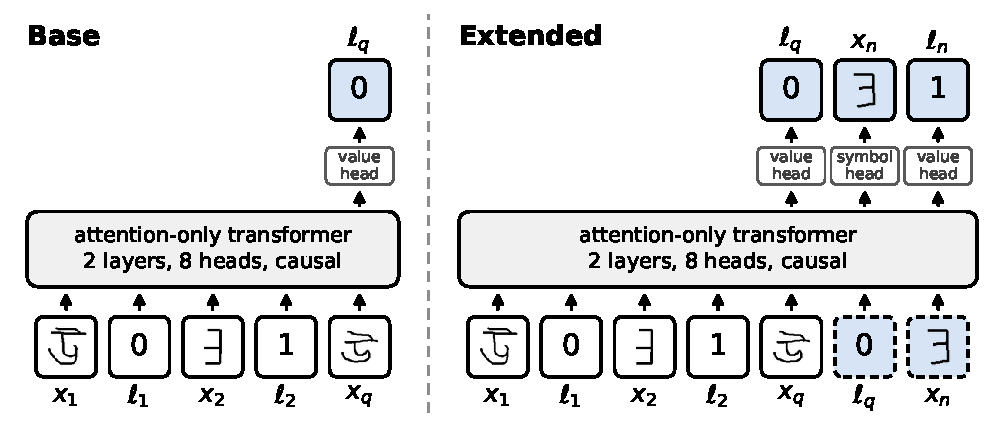
\includegraphics[width=1\columnwidth]{images/model_figure.pdf}
  \caption{Base (left) and extended (right) models.
  The base model predicts the query's label $\ell_q$
  from two symbol--label pairs and query $x_q$.
  The extended model additionally predicts the next
  symbol $x_n$ and its label $\ell_n$.
  Shaded boxes indicate model outputs, while dashed
  inputs represent true tokens during training and
  generated tokens during recursive training.}
  \label{fig:models}
\end{figure}

\subsubsection{Background}
\looseness=-1
\paragraph{Induction heads} The previous-token head copies each symbol into the label that follows it, and the induction head then matches the query against these copies through its key input and copies the matching label to the output \citep{singh2024}. Several induction heads can form and contribute additively \citep{singh2024}, so the circuit can spread across heads rather than rely on one, and interventions on their formation change ICL ability with them \citep{chen2026}.

\paragraph{Model collapse} \citet{shumailov2024} identify sampling error as the primary cause of collapse: finite samples rarely reproduce low-probability events, so the tails of the distribution vanish first, and each model's errors compound in the data of the next. In fine-tuned OPT-125m, preserving 10\% of the original data led to only minor degradation.

\paragraph{Accumulating data} \citet{gerstgrasser2024} found that replacing real data causes test error to grow with every iteration, whereas accumulating synthetic data alongside it keeps the error bounded, across language, diffusion, and autoencoder models. This study tests whether the same contrast holds for the induction circuit.

\section{Methods}
\label{sec:method}

This study varies the share of real data in the training pool and measures its effect on the induction circuit. It uses the setup of \citet{singh2024}, whose circuit is known to form: each sequence holds two exemplar--label pairs and a query, with Omniglot exemplars encoded by a frozen ResNet18 and five labels reassigned per sequence. The model, a causal two-layer attention-only transformer with eight heads per layer, trains on 50 classes and is tested on 100 unseen classes, so that accuracy reflects ICL alone.

\paragraph{Base and extended models} The base model predicts the query's label. The extended model also predicts the next symbol, through a separate symbol head, and that symbol's label (Figure~\ref{fig:models}), so that three tokens per sequence become synthetic rather than one.

\paragraph{Next-symbol selection} By default, the next symbol is a context symbol chosen uniformly, a conservative baseline in which every target remains solvable by the induction circuit. A second condition draws it from all training classes, so that the model must learn an unconditional distribution. Generated tokens are sampled from the softmax at temperature $T$, the source of error described above; argmax removes it and serves as an ablation.

\paragraph{Real-to-synthetic ratio} Each run trains on a fixed pool of $N = 20{,}000$ sequences over six generations, the first on real data. The previous model then regenerates the targets of 0\%, 50\%, 90\%, or 100\% of the pool from their real prompts, where 0\% is a real-only control and 90\% matches the 10\% of real data kept by \citet{shumailov2024}. Accumulation instead keeps every item and adds $N$ synthetic sequences per generation \citep{gerstgrasser2024}, matching 50\% replacement at generation 1, so that keeping earlier data can be separated from the real share itself. A fixed initialisation and training length ensure that conditions differ only in their pool.

\paragraph{Forcing synthetic errors} At $T = 1$, the tuned model regenerates its labels almost perfectly, with 0.01\% wrong after 20 generations, so every ratio yields an essentially real pool. Each regenerating condition is therefore also run at $T = 3$ and $T = 5$, which introduce 0.5\% and 6.5\% wrong labels, so that the ratio acts at a known error rate.

\paragraph{Tuning} As collapse can only alter a circuit that has formed, the learning rate and training length are tuned per model on generation 0, using 1,473 validation classes so that the test classes remain unseen. This gives $\eta = 10^{-4}$ for the base model and $3 \times 10^{-4}$ for the extended model, both for one million sequences.

\paragraph{Burstiness and class distribution} Two sweeps at $T = 1$ test whether properties of the data admit errors without forcing. Burstiness, $B \in \{1, 2, 4\}$, sets how many of eight context items share the query's class: a low $B$ leaves the induction head a single match among many items, which aims to elicit a less confident model whose own errors enter the pool, while a high $B$ provides redundant matches. Zipfian class frequencies, $\alpha \in \{0.5, 1, 1.5\}$, create a long tail of rare symbols.

\paragraph{Circuit analysis} Each generation's model is analysed on the same real sequences, so that changes reflect the model rather than the data. The logit difference measures how strongly the circuit separates the correct label, the number of connections Automatic Circuit DisCovery (ACDC) \citep{conmy2023} keeps at a fixed $\tau = 0.001$ measures whether it stays sparse, and the induction score measures whether the induction head still attends to the match. Patching the previous-token head's output alone into the induction head tests whether the circuit still routes through it, and test accuracy is reported alongside, since it can stay high while the logit difference falls. 

\section{Results}
\label{sec:results}

Table~\ref{tab:summary} summarises every condition at its final generation, and the paragraphs below follow the questions in turn.

\begin{table*}[t]
\centering
\captionsetup{font=sf, width=0.95\linewidth, skip=7pt}
\caption{\looseness=-1 Final generation of each condition. Without forced errors, accuracy holds everywhere except the least bursty context, while the margin falls and the circuit grows. With errors forced at $T = 3$, accumulation keeps accuracy and the induction score near the real-only level for five generations, but declines slowly over 20, whereas each replacement level settles at an accuracy set by its real share. The real-only row never samples and serves as the control at every temperature. $^\dagger$Margin below 1, where the circuit size is less reliable. Induction scores are omitted for eight-item contexts, where they vary between real-only retrains.}
\footnotesize
\begin{tabular}{lccccccccc}
\toprule
 & & Real & Label & \multicolumn{4}{c}{Base model} & \multicolumn{2}{c}{Extended model} \\
\cmidrule(lr){5-8}\cmidrule(lr){9-10}
Condition & Gen. & share & error & Acc. & Margin & Edges & Ind. & Margin & KL \\
\midrule
\multicolumn{10}{l}{\emph{No forced errors} ($T = 1$)} \\
Real only & 5 & 100\% & 0.00 & 0.99 & 20.0 & 19 & 0.97 & 16.0 & 0.00 \\
100\% replaced & 19 & 0\% & 0.01 & 0.99 & 12.5 & 35 & 0.87 & 13.8 & 0.03 \\
Accumulate & 19 & 5\% & 0.00 & 1.00 & 10.4 & 22 & 0.91 & 6.3 & 0.01 \\
100\% replaced, $B = 1$ & 5 & 0\% & 0.06 & 0.75 & 11.0 & 49 & -- & 7.1 & 0.12 \\
100\% replaced, $B = 4$ & 5 & 0\% & 0.00 & 0.99 & 13.2 & 21 & -- & 12.5 & 0.02 \\
\midrule
\multicolumn{10}{l}{\emph{Forced errors} ($T = 3$)} \\
50\% replaced & 5 & 50\% & 0.30 & 0.80 & 3.0 & 198 & 0.84 & 4.6 & 0.00 \\
90\% replaced & 5 & 10\% & 0.66 & 0.38 & 0.6 & 218$^\dagger$ & 0.27 & 0.2 & 0.00 \\
100\% replaced & 5 & 0\% & 0.75 & 0.25 & 0.1 & 209$^\dagger$ & 0.05 & 0.0 & 0.00 \\
Accumulate & 5 & 17\% & 0.31 & 0.99 & 2.1 & 23 & 0.95 & 3.1 & 0.00 \\
\midrule
\multicolumn{10}{l}{\emph{Forced errors over 20 generations} ($T = 3$, base model only)} \\
50\% replaced & 19 & 50\% & 0.33 & 0.78 & 2.7 & 190 & 0.85 & -- & -- \\
90\% replaced & 19 & 10\% & 0.69 & 0.31 & 0.4 & 204$^\dagger$ & 0.16 & -- & -- \\
100\% replaced & 19 & 0\% & 0.79 & 0.19 & 0.1 & 210$^\dagger$ & 0.04 & -- & -- \\
Accumulate & 19 & 5\% & 0.59 & 0.93 & 0.8 & 12$^\dagger$ & 0.80 & -- & -- \\
\bottomrule
\end{tabular}
\label{tab:summary}
\end{table*}

\paragraph{No errors, no collapse} At $T = 1$, the tuned base model regenerates its labels almost exactly, and the 50\%, 90\%, and 100\% replacement runs produce identical models, as does argmax sampling relative to the real-only control. Accuracy therefore stays at 0.99 under every ratio. The circuit nonetheless drifts over 20 generations of full replacement: its margin falls from 19.9 to 12.5 and its ACDC circuit grows from 17 to 35 edges (Figure~\ref{fig:circuits}a--b), whereas the real-only margin varies only between 16.9 and 20.0 across generations. This suggests that the circuit changes before accuracy even when almost no errors enter the data.

\begin{figure}[H]
  \centering
  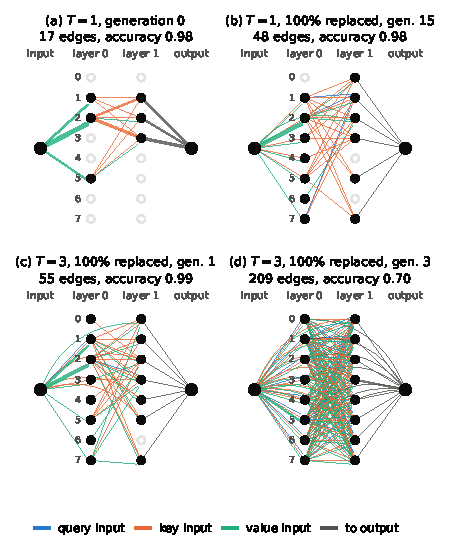
\includegraphics[width=\columnwidth]{images/circuits.pdf}
  \caption{ACDC circuits of the base model on a fixed layout of the input, the eight heads of each layer, and the output, with filled nodes marking heads in the circuit and edge width growing with its effect on the output. At generation 0 (a), the circuit routes the input through the previous-token head A0.2 into the key input of the induction head A1.3. Twenty error-free generations of full replacement (b) double its size while accuracy holds, and forced errors (c) spread it across every head and all three inputs while accuracy is still 0.88. After 20 generations of accumulation with forced errors (d), the circuit has instead contracted to 12 edges, although its margin has fallen below 1.}
  \label{fig:circuits}
\end{figure}

\paragraph{The circuit fails before accuracy} When sampling at $T = 3$ introduces errors, the circuit degrades in a consistent order under full replacement. The margin halves by generation 1, from 19.9 to 10.8, while accuracy holds at 0.99. By generation 2, the circuit has grown from 17 to 188 edges, spreading across every head and into query inputs that the original circuit did not use (Figure~\ref{fig:circuits}c), while accuracy is still 0.88. Accuracy then falls to 0.25 by generation 5, and the induction score falls last, from 0.75 at generation 3 to 0.05, with the previous-token head holding until generation 4. Accuracy then settles near chance, at 0.19 by generation 19, once 79\% of the pool's labels are wrong, close to the 80\% expected from five labels assigned at random. This order is likely because noisy labels make the label only partly predictable from the context, so that the model lowers its confidence and spreads the computation across more connections, consistent with the additive contribution of several heads reported by \citet{singh2024}. % CHECK: mechanism inferred.
The extended model follows the same order, with its circuit growing from 46 to 179 edges while accuracy is still 0.88.

\paragraph{The margin sets the next generation's errors} If the correct label leads each of the four wrong labels by the margin $D_g$ of generation $g$'s model, sampling at temperature $T$ produces wrong labels at a rate of
\begin{equation}
\hat{\epsilon}_{g+1} = \frac{4\,e^{-D_g/T}}{1 + 4\,e^{-D_g/T}}.
\label{eq:error}
\end{equation}
The observed error rate of each generation's new samples closely matches Equation~\ref{eq:error} across both models, both temperatures, and every condition, with a correlation of 0.994 and a mean absolute error of 0.021. At $T = 3$, the generation 0 margin of 19.9 predicts 0.5\% wrong labels, while the margin of 5.3 at generation 2 predicts 41\% against an observed 44\%. The eroding margin is therefore not only a symptom of collapse: it determines how many errors the next generation inherits, which explains why errors compound once they begin.

\paragraph{Retaining real data} Over 20 generations at $T = 3$, each replacement level settles at an accuracy set by its real share, at 0.78 with 50\% real data, 0.31 with 10\%, and 0.19 with none (Figure~\ref{fig:ret-acc}). With 50\% real data, the pool's label error levels off at 33\% and the margin at about 2.7, so that retaining half the real data bounds the collapse but does not prevent the circuit from spreading to 190 edges. Accumulation holds accuracy at 0.97 or above for 15 generations, even though its real share falls to 6\% by then, and at generation 19 it still reaches 0.93 with only 5\% real data, against 0.78 for 50\% replacement. As both conditions hold 50\% real data at generation 1, keeping earlier data appears to matter more than the real share itself, likely because each real prompt keeps its correct label while errors scatter across the four wrong labels. % CHECK: explanation inferred.
However, accumulation delays collapse rather than preventing it: its margin falls steadily from 19.9 to 0.77, the share of wrong labels in its pool rises to 59\%, and accuracy begins to decline once the margin drops below 1 at generation 16. Its circuit contracts to 12 edges rather than spreading (Figure~\ref{fig:circuits}d), although at a margin below 1 this count is less reliable. This contrasts with \citet{gerstgrasser2024}, who found that accumulation keeps the error bounded, and suggests that the margin of the circuit erodes even when its behaviour is protected.

\begin{figure}[H]
  \centering
  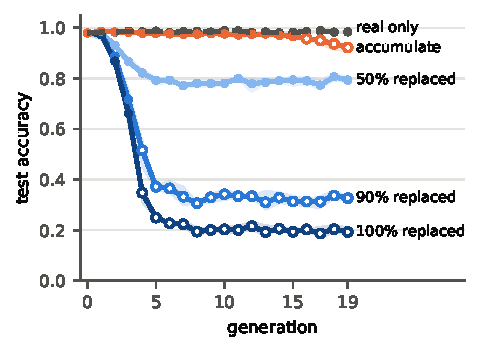
\includegraphics[width=\columnwidth]{images/retention_acc.pdf}
  \caption{Test accuracy of the base model per generation at $T = 3$ for each condition over 20 generations. Each replacement level settles at an accuracy set by its real share, while accumulation stays with the real-only control for 15 generations before declining slowly. Hollow markers indicate a margin below 1.}
  \label{fig:ret-acc}
\end{figure}

\paragraph{Symbol distribution and data properties} The extended model's symbol distribution does not narrow: its divergence from generation 0 stays at or below 0.02, even when 96\% of its next symbols fall outside the context at $T = 3$, so that it collapses through wrong copying rather than a lost tail. Burstiness shows the clearest effect of the data without forced errors. Under full replacement at $T = 1$, the extended model loses 57\%, 39\%, and 14\% of its margin relative to real-only retraining as $B$ rises from 1 to 4, and its symbol divergence falls from 0.12 to 0.02, while only the base model at $B = 1$ admits enough errors to lose accuracy, from 0.83 to 0.75. Redundant matches in the context therefore appear to protect the circuit, likely because they keep the model confident enough that its own samples remain correct. The Zipfian sweeps, in contrast, leave accuracy and the tail mass of the symbol distribution unchanged, likely because the next symbol is copied from real prompts, which preserve rare symbols by construction.

\section{Discussion}
Take a broader perspective of your results and recontextualise them in terms of the field and your community. Your research should aim to be helpful to your community and you will stand better chances of gaining readers if you take this tone. So how has your work helped and what should a reader leave remembering?

\section{Acknowledgements (Not in Page Limit -- you will probably not have one)}
Computations were performed using High Performance Computing infrastructure provided by the Mathematical Sciences Support Unit at the University of the Witwatersrand.

\section{Contribution Statements (Not in Page Limit)}
This can be different to the preliminary one but the authors must stay the same. Please ensure that all group members agree on what is said here.

Do not forget to include the NeurIPS Checklist and the Wits Science Faculty AI Ethics Form.

\bibliographystyle{apacite}

\setlength{\bibleftmargin}{.125in}
\setlength{\bibindent}{-\bibleftmargin}

\bibliography{ccn_style} % must match your .bib file name, e.g. references for references.bib

\newpage
% NeurIPS 2024 paper checklist, from the lecturer's NeurIPS_2024_checklist/neurips_2024.tex
% (the body between \begin{document} and \end{document}). The answer macros it uses are
% defined in the ccn_style.tex preamble, matching neurips_2024.sty.

\appendix

\section*{NeurIPS Paper Checklist}



\begin{enumerate}

\item {\bf Claims}
    \item[] Question: Do the main claims made in the abstract and introduction accurately reflect the paper's contributions and scope?
    \item[] Answer: \answerYes{}
    \item[] Justification: The abstract states the three main findings of this study, and the introduction the question that they answer, namely that, once synthetic data carry errors, the model's confidence and its induction circuit change before its accuracy does, that the margin of each generation's model predicts the error rate of the next generation's data, and that retaining real data limits how far accuracy falls while accumulation delays its decline without stopping the margin's erosion. Each claim is supported in the Results (Table~\ref{tab:summary}, Figures~\ref{fig:circuits} and~\ref{fig:head}, and Equation~\ref{eq:error}), and the abstract states that errors were forced by raising the sampling temperature, so that the scope of the claims is clear.
    \item[] Guidelines:
    \begin{itemize}
        \item The answer NA means that the abstract and introduction do not include the claims made in the paper.
        \item The abstract and/or introduction should clearly state the claims made, including the contributions made in the paper and important assumptions and limitations. A No or NA answer to this question will not be perceived well by the reviewers. 
        \item The claims made should match theoretical and experimental results, and reflect how much the results can be expected to generalize to other settings. 
        \item It is fine to include aspirational goals as motivation as long as it is clear that these goals are not attained by the paper. 
    \end{itemize}

\item {\bf Limitations}
    \item[] Question: Does the paper discuss the limitations of the work performed by the authors?
    \item[] Answer: \answerYes{}
    \item[] Justification: The Discussion states that errors were forced by raising the sampling temperature rather than arising from a weaker model, and that the training length was fixed while the accumulated pool grew 20-fold. The Results separate the share of the extended model's off-context next symbols caused by the temperature from the share its later models learn. In addition, the Results note that circuit sizes are less reliable once the margin falls below 1 (Table~\ref{tab:summary}). This study is also limited to a single two-layer attention-only model and a single synthetic task.
    \item[] Guidelines:
    \begin{itemize}
        \item The answer NA means that the paper has no limitation while the answer No means that the paper has limitations, but those are not discussed in the paper. 
        \item The authors are encouraged to create a separate "Limitations" section in their paper.
        \item The paper should point out any strong assumptions and how robust the results are to violations of these assumptions (e.g., independence assumptions, noiseless settings, model well-specification, asymptotic approximations only holding locally). The authors should reflect on how these assumptions might be violated in practice and what the implications would be.
        \item The authors should reflect on the scope of the claims made, e.g., if the approach was only tested on a few datasets or with a few runs. In general, empirical results often depend on implicit assumptions, which should be articulated.
        \item The authors should reflect on the factors that influence the performance of the approach. For example, a facial recognition algorithm may perform poorly when image resolution is low or images are taken in low lighting. Or a speech-to-text system might not be used reliably to provide closed captions for online lectures because it fails to handle technical jargon.
        \item The authors should discuss the computational efficiency of the proposed algorithms and how they scale with dataset size.
        \item If applicable, the authors should discuss possible limitations of their approach to address problems of privacy and fairness.
        \item While the authors might fear that complete honesty about limitations might be used by reviewers as grounds for rejection, a worse outcome might be that reviewers discover limitations that aren't acknowledged in the paper. The authors should use their best judgment and recognize that individual actions in favor of transparency play an important role in developing norms that preserve the integrity of the community. Reviewers will be specifically instructed to not penalize honesty concerning limitations.
    \end{itemize}

\item {\bf Theory Assumptions and Proofs}
    \item[] Question: For each theoretical result, does the paper provide the full set of assumptions and a complete (and correct) proof?
    \item[] Answer: \answerNA{}
    \item[] Justification: This study contains no theorems. Equation~\ref{eq:error} follows directly from the softmax under the approximation stated with it, namely that the measured margin against the other context label holds against all four wrong labels, and is tested empirically rather than proven.
    \item[] Guidelines:
    \begin{itemize}
        \item The answer NA means that the paper does not include theoretical results. 
        \item All the theorems, formulas, and proofs in the paper should be numbered and cross-referenced.
        \item All assumptions should be clearly stated or referenced in the statement of any theorems.
        \item The proofs can either appear in the main paper or the supplemental material, but if they appear in the supplemental material, the authors are encouraged to provide a short proof sketch to provide intuition. 
        \item Inversely, any informal proof provided in the core of the paper should be complemented by formal proofs provided in appendix or supplemental material.
        \item Theorems and Lemmas that the proof relies upon should be properly referenced. 
    \end{itemize}

    \item {\bf Experimental Result Reproducibility}
    \item[] Question: Does the paper fully disclose all the information needed to reproduce the main experimental results of the paper to the extent that it affects the main claims and/or conclusions of the paper (regardless of whether the code and data are provided or not)?
    \item[] Answer: \answerYes{}
    \item[] Justification: The Methods specify the task, architecture, class splits, pool size, real-to-synthetic ratios, sampling temperatures, tuned learning rates, training length, and Automatic Circuit DisCovery (ACDC) threshold. The remaining settings, namely the Adam optimiser, a batch size of 32, a model width of 64, and the three seed pairs of the initialisation and training data, are fixed in the released run scripts, so that each run can be repeated under the same configuration.
    \item[] Guidelines:
    \begin{itemize}
        \item The answer NA means that the paper does not include experiments.
        \item If the paper includes experiments, a No answer to this question will not be perceived well by the reviewers: Making the paper reproducible is important, regardless of whether the code and data are provided or not.
        \item If the contribution is a dataset and/or model, the authors should describe the steps taken to make their results reproducible or verifiable. 
        \item Depending on the contribution, reproducibility can be accomplished in various ways. For example, if the contribution is a novel architecture, describing the architecture fully might suffice, or if the contribution is a specific model and empirical evaluation, it may be necessary to either make it possible for others to replicate the model with the same dataset, or provide access to the model. In general. releasing code and data is often one good way to accomplish this, but reproducibility can also be provided via detailed instructions for how to replicate the results, access to a hosted model (e.g., in the case of a large language model), releasing of a model checkpoint, or other means that are appropriate to the research performed.
        \item While NeurIPS does not require releasing code, the conference does require all submissions to provide some reasonable avenue for reproducibility, which may depend on the nature of the contribution. For example
        \begin{enumerate}
            \item If the contribution is primarily a new algorithm, the paper should make it clear how to reproduce that algorithm.
            \item If the contribution is primarily a new model architecture, the paper should describe the architecture clearly and fully.
            \item If the contribution is a new model (e.g., a large language model), then there should either be a way to access this model for reproducing the results or a way to reproduce the model (e.g., with an open-source dataset or instructions for how to construct the dataset).
            \item We recognize that reproducibility may be tricky in some cases, in which case authors are welcome to describe the particular way they provide for reproducibility. In the case of closed-source models, it may be that access to the model is limited in some way (e.g., to registered users), but it should be possible for other researchers to have some path to reproducing or verifying the results.
        \end{enumerate}
    \end{itemize}


\item {\bf Open access to data and code}
    \item[] Question: Does the paper provide open access to the data and code, with sufficient instructions to faithfully reproduce the main experimental results, as described in supplemental material?
    \item[] Answer: \answerYes{}
    \item[] Justification: The code, the preprocessed Omniglot features, and the scripts that run every experiment and produce every figure are available at \url{https://github.com/froggomelo/nlp-project-1}. The repository's README specifies the environment and the exact command for each experiment.
    \item[] Guidelines:
    \begin{itemize}
        \item The answer NA means that paper does not include experiments requiring code.
        \item Please see the NeurIPS code and data submission guidelines (\url{https://nips.cc/public/guides/CodeSubmissionPolicy}) for more details.
        \item While we encourage the release of code and data, we understand that this might not be possible, so “No” is an acceptable answer. Papers cannot be rejected simply for not including code, unless this is central to the contribution (e.g., for a new open-source benchmark).
        \item The instructions should contain the exact command and environment needed to run to reproduce the results. See the NeurIPS code and data submission guidelines (\url{https://nips.cc/public/guides/CodeSubmissionPolicy}) for more details.
        \item The authors should provide instructions on data access and preparation, including how to access the raw data, preprocessed data, intermediate data, and generated data, etc.
        \item The authors should provide scripts to reproduce all experimental results for the new proposed method and baselines. If only a subset of experiments are reproducible, they should state which ones are omitted from the script and why.
        \item At submission time, to preserve anonymity, the authors should release anonymized versions (if applicable).
        \item Providing as much information as possible in supplemental material (appended to the paper) is recommended, but including URLs to data and code is permitted.
    \end{itemize}


\item {\bf Experimental Setting/Details}
    \item[] Question: Does the paper specify all the training and test details (e.g., data splits, hyperparameters, how they were chosen, type of optimizer, etc.) necessary to understand the results?
    \item[] Answer: \answerYes{}
    \item[] Justification: The Methods state that the model trains on 50 Omniglot classes and is tested on 100 unseen classes, so that test accuracy reflects ICL alone. The learning rate and training length were tuned per model on 1,473 separate validation classes, so that the test classes remain unseen during tuning, and the chosen values are reported.
    \item[] Guidelines:
    \begin{itemize}
        \item The answer NA means that the paper does not include experiments.
        \item The experimental setting should be presented in the core of the paper to a level of detail that is necessary to appreciate the results and make sense of them.
        \item The full details can be provided either with the code, in appendix, or as supplemental material.
    \end{itemize}

\item {\bf Experiment Statistical Significance}
    \item[] Question: Does the paper report error bars suitably and correctly defined or other appropriate information about the statistical significance of the experiments?
    \item[] Answer: \answerYes{}
    \item[] Justification: Each condition of Table~\ref{tab:summary} was run with three seeds of the initialisation and training data, and the table reports the mean $\pm$ the standard deviation over seeds. Figure~\ref{fig:head} shades the range across seeds, the text gives means and, where a claim depends on it, the worst seed, and the fit of Equation~\ref{eq:error} is reported as a correlation and an average absolute gap across every generation and condition.
    \item[] Guidelines:
    \begin{itemize}
        \item The answer NA means that the paper does not include experiments.
        \item The authors should answer "Yes" if the results are accompanied by error bars, confidence intervals, or statistical significance tests, at least for the experiments that support the main claims of the paper.
        \item The factors of variability that the error bars are capturing should be clearly stated (for example, train/test split, initialization, random drawing of some parameter, or overall run with given experimental conditions).
        \item The method for calculating the error bars should be explained (closed form formula, call to a library function, bootstrap, etc.)
        \item The assumptions made should be given (e.g., Normally distributed errors).
        \item It should be clear whether the error bar is the standard deviation or the standard error of the mean.
        \item It is OK to report 1-sigma error bars, but one should state it. The authors should preferably report a 2-sigma error bar than state that they have a 96\% CI, if the hypothesis of Normality of errors is not verified.
        \item For asymmetric distributions, the authors should be careful not to show in tables or figures symmetric error bars that would yield results that are out of range (e.g. negative error rates).
        \item If error bars are reported in tables or plots, The authors should explain in the text how they were calculated and reference the corresponding figures or tables in the text.
    \end{itemize}

\item {\bf Experiments Compute Resources}
    \item[] Question: For each experiment, does the paper provide sufficient information on the computer resources (type of compute workers, memory, time of execution) needed to reproduce the experiments?
    \item[] Answer: \answerYes{}
    \item[] Justification: Every experiment was run on the CPU of a single desktop computer (AMD Ryzen 7 7800X3D, 32 GB of RAM). Training on one million sequences took approximately 2.2 minutes, so that the 580 trainings of the full run script take roughly a day, with circuit discovery and the longer eight-item contexts adding to this. Repeating the 14 runs of Table~\ref{tab:summary} for two more seeds added 28 runs of 20 generations, or 560 trainings. Development runs not reported in this study used additional compute of a similar scale.
    \item[] Guidelines:
    \begin{itemize}
        \item The answer NA means that the paper does not include experiments.
        \item The paper should indicate the type of compute workers CPU or GPU, internal cluster, or cloud provider, including relevant memory and storage.
        \item The paper should provide the amount of compute required for each of the individual experimental runs as well as estimate the total compute. 
        \item The paper should disclose whether the full research project required more compute than the experiments reported in the paper (e.g., preliminary or failed experiments that didn't make it into the paper). 
    \end{itemize}
    
\item {\bf Code Of Ethics}
    \item[] Question: Does the research conducted in the paper conform, in every respect, with the NeurIPS Code of Ethics \url{https://neurips.cc/public/EthicsGuidelines}?
    \item[] Answer: \answerYes{}
    \item[] Justification: This study uses a public dataset of handwritten characters and small models trained for analysis. It involves no human subjects or personal data and releases no model with a risk of misuse.
    \item[] Guidelines:
    \begin{itemize}
        \item The answer NA means that the authors have not reviewed the NeurIPS Code of Ethics.
        \item If the authors answer No, they should explain the special circumstances that require a deviation from the Code of Ethics.
        \item The authors should make sure to preserve anonymity (e.g., if there is a special consideration due to laws or regulations in their jurisdiction).
    \end{itemize}


\item {\bf Broader Impacts}
    \item[] Question: Does the paper discuss both potential positive societal impacts and negative societal impacts of the work performed?
    \item[] Answer: \answerNA{}
    \item[] Justification: This study is foundational research on a small model trained on a synthetic task and has no direct path to harmful applications. Its one implied application, namely using the margin or an identified circuit to flag collapse before accuracy falls, is a positive use and is considered in the Discussion.
    \item[] Guidelines:
    \begin{itemize}
        \item The answer NA means that there is no societal impact of the work performed.
        \item If the authors answer NA or No, they should explain why their work has no societal impact or why the paper does not address societal impact.
        \item Examples of negative societal impacts include potential malicious or unintended uses (e.g., disinformation, generating fake profiles, surveillance), fairness considerations (e.g., deployment of technologies that could make decisions that unfairly impact specific groups), privacy considerations, and security considerations.
        \item The conference expects that many papers will be foundational research and not tied to particular applications, let alone deployments. However, if there is a direct path to any negative applications, the authors should point it out. For example, it is legitimate to point out that an improvement in the quality of generative models could be used to generate deepfakes for disinformation. On the other hand, it is not needed to point out that a generic algorithm for optimizing neural networks could enable people to train models that generate Deepfakes faster.
        \item The authors should consider possible harms that could arise when the technology is being used as intended and functioning correctly, harms that could arise when the technology is being used as intended but gives incorrect results, and harms following from (intentional or unintentional) misuse of the technology.
        \item If there are negative societal impacts, the authors could also discuss possible mitigation strategies (e.g., gated release of models, providing defenses in addition to attacks, mechanisms for monitoring misuse, mechanisms to monitor how a system learns from feedback over time, improving the efficiency and accessibility of ML).
    \end{itemize}
    
\item {\bf Safeguards}
    \item[] Question: Does the paper describe safeguards that have been put in place for responsible release of data or models that have a high risk for misuse (e.g., pretrained language models, image generators, or scraped datasets)?
    \item[] Answer: \answerNA{}
    \item[] Justification: The released models are two-layer transformers trained on Omniglot features and therefore pose no risk of misuse.
    \item[] Guidelines:
    \begin{itemize}
        \item The answer NA means that the paper poses no such risks.
        \item Released models that have a high risk for misuse or dual-use should be released with necessary safeguards to allow for controlled use of the model, for example by requiring that users adhere to usage guidelines or restrictions to access the model or implementing safety filters. 
        \item Datasets that have been scraped from the Internet could pose safety risks. The authors should describe how they avoided releasing unsafe images.
        \item We recognize that providing effective safeguards is challenging, and many papers do not require this, but we encourage authors to take this into account and make a best faith effort.
    \end{itemize}

\item {\bf Licenses for existing assets}
    \item[] Question: Are the creators or original owners of assets (e.g., code, data, models), used in the paper, properly credited and are the license and terms of use explicitly mentioned and properly respected?
    \item[] Answer: \answerYes{}
    \item[] Justification: Omniglot \citep{lake2015} is used under the MIT License, and the ResNet18 ImageNet weights \citep{he2016} are taken from torchvision under the BSD-3-Clause License. Circuit discovery uses ACDC \citep{conmy2023} through the auto-circuit (version 1.0.1) and TransformerLens (version 2.9.0) libraries, both under the MIT License. The training code extends the released codebase of \citet{singh2024}, which is credited in the repository.
    \item[] Guidelines:
    \begin{itemize}
        \item The answer NA means that the paper does not use existing assets.
        \item The authors should cite the original paper that produced the code package or dataset.
        \item The authors should state which version of the asset is used and, if possible, include a URL.
        \item The name of the license (e.g., CC-BY 4.0) should be included for each asset.
        \item For scraped data from a particular source (e.g., website), the copyright and terms of service of that source should be provided.
        \item If assets are released, the license, copyright information, and terms of use in the package should be provided. For popular datasets, \url{paperswithcode.com/datasets} has curated licenses for some datasets. Their licensing guide can help determine the license of a dataset.
        \item For existing datasets that are re-packaged, both the original license and the license of the derived asset (if it has changed) should be provided.
        \item If this information is not available online, the authors are encouraged to reach out to the asset's creators.
    \end{itemize}

\item {\bf New Assets}
    \item[] Question: Are new assets introduced in the paper well documented and is the documentation provided alongside the assets?
    \item[] Answer: \answerYes{}
    \item[] Justification: The released code is documented in the repository's README and in the files of \texttt{docs/}, which describe each experiment, its settings, and how it is reproduced. No data were collected from people, so that consent does not apply.
    \item[] Guidelines:
    \begin{itemize}
        \item The answer NA means that the paper does not release new assets.
        \item Researchers should communicate the details of the dataset/code/model as part of their submissions via structured templates. This includes details about training, license, limitations, etc. 
        \item The paper should discuss whether and how consent was obtained from people whose asset is used.
        \item At submission time, remember to anonymize your assets (if applicable). You can either create an anonymized URL or include an anonymized zip file.
    \end{itemize}

\item {\bf Crowdsourcing and Research with Human Subjects}
    \item[] Question: For crowdsourcing experiments and research with human subjects, does the paper include the full text of instructions given to participants and screenshots, if applicable, as well as details about compensation (if any)? 
    \item[] Answer: \answerNA{}
    \item[] Justification: This study involves neither crowdsourcing nor research with human subjects.
    \item[] Guidelines:
    \begin{itemize}
        \item The answer NA means that the paper does not involve crowdsourcing nor research with human subjects.
        \item Including this information in the supplemental material is fine, but if the main contribution of the paper involves human subjects, then as much detail as possible should be included in the main paper. 
        \item According to the NeurIPS Code of Ethics, workers involved in data collection, curation, or other labor should be paid at least the minimum wage in the country of the data collector. 
    \end{itemize}

\item {\bf Institutional Review Board (IRB) Approvals or Equivalent for Research with Human Subjects}
    \item[] Question: Does the paper describe potential risks incurred by study participants, whether such risks were disclosed to the subjects, and whether Institutional Review Board (IRB) approvals (or an equivalent approval/review based on the requirements of your country or institution) were obtained?
    \item[] Answer: \answerNA{}
    \item[] Justification: This study involves neither crowdsourcing nor research with human subjects.
    \item[] Guidelines:
    \begin{itemize}
        \item The answer NA means that the paper does not involve crowdsourcing nor research with human subjects.
        \item Depending on the country in which research is conducted, IRB approval (or equivalent) may be required for any human subjects research. If you obtained IRB approval, you should clearly state this in the paper. 
        \item We recognize that the procedures for this may vary significantly between institutions and locations, and we expect authors to adhere to the NeurIPS Code of Ethics and the guidelines for their institution. 
        \item For initial submissions, do not include any information that would break anonymity (if applicable), such as the institution conducting the review.
    \end{itemize}

\end{enumerate}




\includepdf[pages=-]{ai_dec.pdf}

\end{document}